\tikzset{every picture/.style={line width=0.75pt}} %set default line width to 0.75pt        

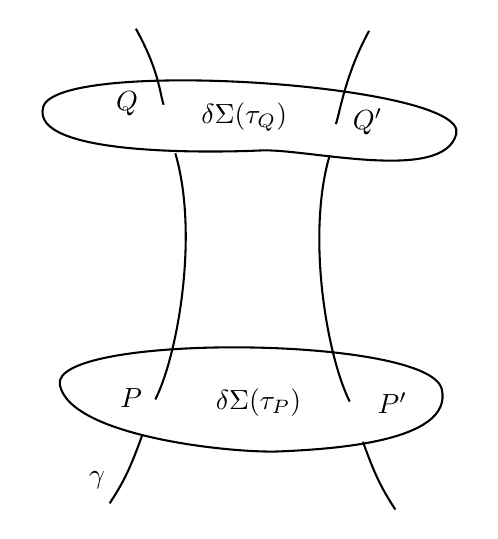
\begin{tikzpicture}[x=0.75pt,y=0.75pt,yscale=-1,xscale=1]
	%uncomment if require: \path (0,240); %set diagram left start at 0, and has height of 240
	
	%Shape: Polygon Curved [id:ds9889967043155199] 
	\draw   (228.37,40.65) .. controls (235.37,16.65) and (433.37,29.65) .. (427.37,53.65) .. controls (421.37,77.65) and (355.37,60.65) .. (333.37,61.65) .. controls (311.37,62.65) and (221.37,64.65) .. (228.37,40.65) -- cycle ;
	%Shape: Polygon Curved [id:ds13480469303111686] 
	\draw   (236.37,174.65) .. controls (231.37,149.65) and (414.37,150.65) .. (420.37,176.65) .. controls (426.37,202.65) and (364.37,205.65) .. (342.37,206.65) .. controls (320.37,207.65) and (241.37,199.65) .. (236.37,174.65) -- cycle ;
	%Curve Lines [id:da4172336256165927] 
	\draw    (273,3) .. controls (284.37,23.65) and (284.37,33.65) .. (286.37,39.65) ;
	%Curve Lines [id:da15007501193341932] 
	\draw    (292,63) .. controls (303.37,101.65) and (293.37,159.65) .. (282.37,181.65) ;
	%Curve Lines [id:da33073366226575596] 
	\draw    (276,199) .. controls (271.37,211.65) and (268.37,219.65) .. (260.37,231.65) ;
	%Curve Lines [id:da8256739981494945] 
	\draw    (385.38,4) .. controls (374.02,24.65) and (371.37,42.97) .. (369.37,48.97) ;
	%Curve Lines [id:da9874647131889831] 
	\draw    (366.38,64) .. controls (355.02,102.65) and (365.02,160.65) .. (376.02,182.65) ;
	%Curve Lines [id:da16314709480723044] 
	\draw    (382.38,202) .. controls (387.02,214.65) and (390.02,222.65) .. (398.02,234.65) ;
	
	% Text Node
	\draw (262,32) node [anchor=north west][inner sep=0.75pt]    {$Q$};
	% Text Node
	\draw (376,40) node [anchor=north west][inner sep=0.75pt]    {$Q'$};
	% Text Node
	\draw (264,175) node [anchor=north west][inner sep=0.75pt]    {$P$};
	% Text Node
	\draw (388,177) node [anchor=north west][inner sep=0.75pt]    {$P'$};
	% Text Node
	\draw (303,37) node [anchor=north west][inner sep=0.75pt]    {$\delta \Sigma ( \tau _{Q})$};
	% Text Node
	\draw (310,175) node [anchor=north west][inner sep=0.75pt]    {$\delta \Sigma ( \tau _{P})$};
	% Text Node
	\draw (249,215) node [anchor=north west][inner sep=0.75pt]    {$\gamma $};
	
	
\end{tikzpicture}